%% ============================================================================
\section{Empirical Evaluation}
\label{sec:eval}
%% ============================================================================

In this section, we evaluate the theoretical predictions of §\ref{sec:framework} in two complementary settings. 
On LoCoBench (§\ref{sec:experiments}), a controlled benchmark of coherence ladders with 
gold relation graphs, responses differ only in their argument structure while preserving 
the underlying claims and verdicts. This lets us test each prediction directly, both under 
gold graphs and under automatically mined graphs, and compare LCS against text-based metrics 
and LLM judges. On natural text (§\ref{sec:exp-external}), we use three existing datasets 
together with a corpus of rated student essays. These datasets do not provide human 
annotations of \emph{logical coherence}; instead, they are labelled for discourse coherence, 
inserted contradictions, or overall essay quality. 
We therefore test four properties that the framework implies: $\LCS$ is not a proxy for discourse 
coherence, falls when a detected contradiction is added, ignores the order of paragraphs, and 
tracks the quality of arguments beyond confounds such as length.


\paragraph{Common setup.} Unless stated otherwise, relations are extracted with the 
graph-level miner (§\ref{sec:mining}) using GPT-6\footnote{In all our experiments we used GPT-6-Sol.}, 
which was not involved in constructing 
LoCoBench; results with gpt-oss-120b are also reported. For LoCoBench, we additionally 
evaluate the pairwise miner (window size $4$) with gpt-oss-120b and Llama-3.3-70B. We use 
flat (or uniform) claim priors throughout.


\subsection{Controlled Evaluation on LoCoBench}
\label{sec:experiments}
\label{sec-experiments}
\label{sec-locobench}

\paragraph{Data.} LoCoBench \citep{anonlocobench} builds \emph{coherence ladders}: responses over
fixed claims that differ only in argument structure, with gold relation graphs. Each of its
\sThreeFamilies{} families is an expert answer written as a template with \emph{slots}; a slot
joins two claims, and its fillers draw no link, a support or a conflict between them. A ladder's
three rungs $\rho_0,\rho_1,\rho_2$ splice different fillers into the template, so they share every
other word, every claim and every verdict. Three ladder types are declared increasing: \cp{conflict}
removes conflicts between true claims, \cp{chain} adds entailments between them, and \cp{sign} goes
from deriving a false claim, through no link, to refuting it. Two are declared invariant: \cp{order}
permutes paragraphs and \cp{control} rewords one entailment. A three-vendor model committee reads
the gold relations pair by pair, and a ladder is admitted only if its gold graphs are ordered as
declared, by at least $0.05$ nats in $\Lambda$. The \sThreeLadders{} ladders have \sThreeItems{}
responses of 12--14 claims, two or three of them false; factuality labels give the verdict world and
stance the asserted world. Each ladder gives three rung pairs, so the \sThreeNConflict{} ladders of
each increasing type give $180$ pairs (App.~\ref{sec-full-locobench} and supplementary materials).

\paragraph{Setup.} The ladders induce \sThreeNIncPairs{} \emph{Increase} and \sThreeNInvPairs{}
\emph{Invariance} comparisons. Every score must rise on an Increase pair and stay equal on an
Invariance pair, up to a relative tie tolerance of $\sThreeRelTie$ (App.~\ref{app:setup-details}).
An \emph{arm} fixes the graph source: the \cp{gold} relations or one of four mining
configurations, each read at the verdict world (our default) and at the asserted world. On every
arm we also score $\LCS$'s three simplifications over the same graphs (\S\ref{sec:decomp}): the
signed weight sum $\Ssum$, the linear evidence $\Llin$ and the independent evidence $\Lambda^{\perp}$. Text baselines are length, DiscoScore (RC, LC, entity graph)
\citep{discoscore}, and judges using G-Eval \citep{geval} and a direct 1--5 rating of logical
coherence, averaged over five runs with GPT-6 and gpt-oss-120b; the judges see the response only.
Baselines that read only the claims tie on every pair (App.~\ref{app:results}). Error bars are 95\%
percentile-bootstrap intervals over families.

\begin{figure*}[t]
\centering
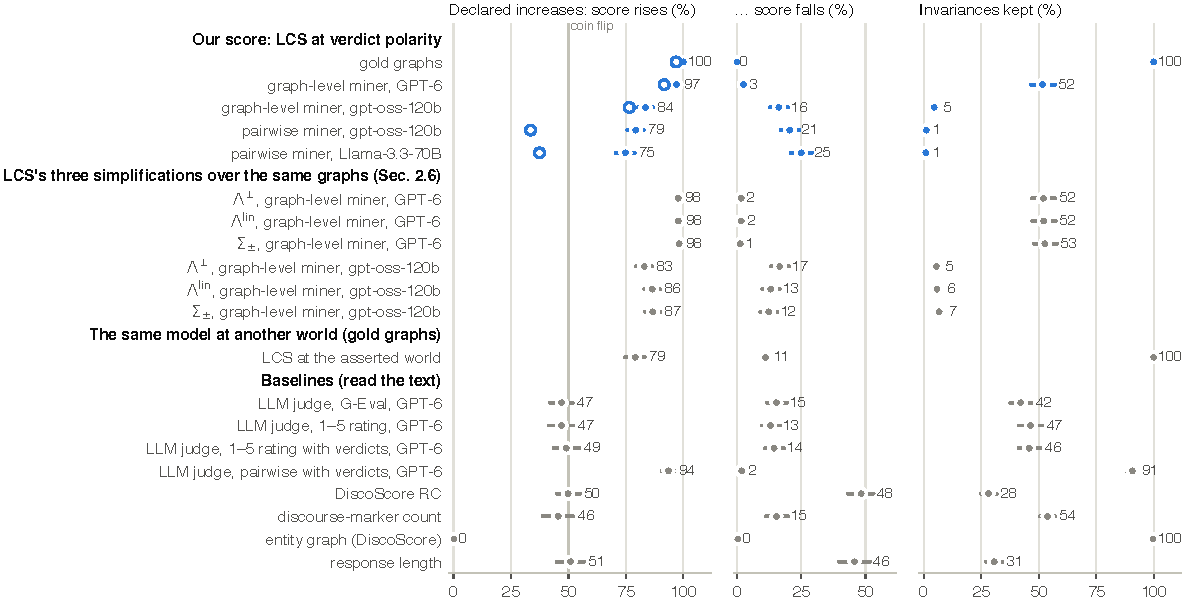
\includegraphics[width=1\textwidth]{figures/fig_ladders.pdf}
\caption{\textbf{Every score on LoCoBench's \sThreeNIncPairs{} declared increases and
\sThreeNInvPairs{} declared invariances.} \emph{Left:} share of Increase pairs on which the score
rises strictly; \emph{middle:} share on which it falls (the rest are ties). A score that ignores the
edits gets $0\%$ in both, a random one about $50\%$ in both. \emph{Right:} share of Invariance
pairs on which the score stays equal. \emph{Blue:}
$\LCS$ at the verdict world, on gold and mined graphs; hollow blue markers give the share that rises
by more than $\tau$. Judges average five runs, the verdict-aware
absolute judge three. \emph{Gray:} $\LCS$'s three simplifications over the graph-level arms'
graphs (all arms in Table~\ref{tab:signed}): the independent evidence $\Lambda^{\perp}$ (no
interaction), the linear evidence $\Llin$ (first order) and the signed weight sum $\Ssum$
(\S\ref{sec:decomp}); $\LCS$ at the asserted world; and the baselines. The entity graph reads the text but scores only nouns shared by nearby sentences, so it too
almost never moves.}
\label{fig:ladders}
\end{figure*}



\label{sec:exp-gold}
\label{sec:exp-mined}
\label{sec:exp-polarity}
\label{sec:exp-baselines}

\paragraph{Gold graphs check the implementation.} On gold graphs $\LCS$ satisfies all
\sThreeNIncPairs{} Increase and all \sThreeNInvPairs{} Invariance pairs (Figure~\ref{fig:ladders},
top row). This holds by construction, since the admission gate keeps only ladders whose gold
graphs are ordered, and it confirms that the implementation matches Theorem~\ref{thm:mono}.

\paragraph{The verdicts are needed.} At the \emph{asserted} world, which takes claims as the response
states them, gold graphs satisfy every \cp{conflict} and \cp{chain} pair but only
\sThreeGoldLamASign{} \cp{sign} pairs, as any signed score does: a derived falsehood counts as a
support there (App.~\ref{app:asserted-sign}).

\paragraph{Mined graphs: extraction sets the rate.} With mined graphs $\LCS$ rises on
\sThreeGraphGptLamIncPct\% (GPT-6 graph-level miner) to \sThreePairLlamaLamIncPct\% (pairwise Llama)
of the increases, and by more than $\tau=\sThreeTol$ on \sThreeGraphGptLamIncTolPct\% to
\sThreePairOssLamIncTolPct\%. Theorem~\ref{thm:mono} covers only pairs whose extracted graphs are
ordered as declared (\sThreeGraphGptDomForward{} of \sThreeNIncPairs{} with GPT-6, \sThreePairOssDomForward{}
with each pairwise miner), where $\LCS$ always rises (Figure~\ref{fig:dominance}). A weaker
graph-level miner from outside the committee's vendors (Llama-3.3-70B, \subLadders{} ladders) reaches
pair-level F1 \subLlamaPairF{} against \subGptPairF{} for GPT-6, and $\LCS$ rises on \subLlamaLcsInc\%
of its increases against \subGptLcsInc\%: results depend on the miner.

\begin{table}[t]
\centering\footnotesize
\setlength{\tabcolsep}{2.4pt}
\begin{tabularx}{\columnwidth}{@{}>{\raggedright\arraybackslash}Xcccc@{}}
\toprule
& $\Ssum$ & $\Llin$ & $\Lambda^{\perp}$ & $\LCS$ \\
\midrule
\multicolumn{5}{@{}l}{\emph{What each keeps} (\S\ref{sec:decomp})}\\
Violation outweighs support & -- & \checkmark & \checkmark & \checkmark \\
Curvature of $\lambda_r$ & -- & -- & \checkmark & \checkmark \\
Relations interact (A2) & -- & -- & -- & \checkmark \\
Range, unit & $\mathbb{R}$ & $\mathbb{R}$, nats & $\mathbb{R}$, nats & $(0,1)$, odds \\
\midrule
\multicolumn{5}{@{}l}{\emph{By construction} (\% of gold graphs; App.~\ref{app:results})}\\
Two halves score as the whole & \zsEqvSum & \zsEqvLin & \zsEqvIndep & \zsEqvLcs \\
Repetition counts less & \zsRepSum & \zsRepLin & \zsRepIndep & \zsRepLcs \\
Contested premise counts less & \zsDoubtSum & \zsDoubtLin & \zsDoubtIndep & \zsDoubtLcs \\
\midrule
\multicolumn{5}{@{}l}{\emph{LoCoBench increases satisfied} (\%)}\\
Gold graphs & \sThreeGoldWsumIncPct & \sThreeGoldLinIncPct & \sThreeGoldIndepIncPct & \sThreeGoldLamIncPct \\
Gold, 20\% of verdicts flipped & \vnWsumIncTwenty & \vnLinIncTwenty & \vnIndepIncTwenty & \vnLcsIncTwenty \\
GPT-6 graphs & \dcAttrWsum & \dcAttrLin & \dcAttrIndep & \dcAttrLcs \\
GPT-6, verifier's verdicts & \vfGptMinedWsumInc & \vfGptMinedLinInc & \vfGptMinedIndepInc & \vfGptMinedLcsInc \\
\midrule
\multicolumn{5}{@{}l}{\emph{ExpertQA} (\dcCountN{} answers, expert verdicts)}\\
$\rho$ with number of relations & $\dcCountWsumNrel$ & $\dcCountLinNrel$ & $\dcCountIndepNrel$ & $\dcCountLcsNrel$ \\
\bottomrule
\end{tabularx}
\caption{\textbf{$\LCS$ beside its three simplifications} (Prop.~\ref{prop:decomp}). Left to
right, each column adds one ingredient: the support/violation asymmetry ($\Llin$), the curvature of
the per-relation evidence $\lambda_r$ ($\Lambda^{\perp}=\sum_r\lambda_r$), and the interaction
$I_\R$ ($\LCS$). All four satisfy A1 and A3. The constructed edits hold or fail by definition; they
show what each score encodes, not how accurate it is (\zsEqvN{} gold graphs, \zsDoubtN{} for the
contested premise). Rows are read at the verdict world.}
\label{tab:three}
\end{table}

\paragraph{Where the four scores differ.} With correct verdicts all four satisfy every gold
increase (Table~\ref{tab:three}): each rung changes one relation's sign, which they read alike, and
the interaction is small on these graphs (median $|I_\R|=\dcIGoldAbsMedian$ nats against
$\dcLamGoldAbsMedian$ for $|\Lambda|$; Figure~\ref{fig:decomp}). Each step of the chain
$\Ssum\to\Llin\to\Lambda^{\perp}\to\LCS$ adds one ingredient, and the data separate them.
\begin{itemize}[leftmargin=1.2em,itemsep=1pt,topsep=2pt]
\item \textbf{The asymmetry decides the wrong-verdict case, and it is first order.} With 20\% of
  the verdicts flipped, $\Llin$, $\Lambda^{\perp}$ and $\LCS$ keep exactly the same increases (the
  curvature and interaction steps change none, \asapCI{\vnDiffILLoIncTwenty}{\vnDiffILHiIncTwenty}
  and \asapCI{\vnDiffLILoIncTwenty}{\vnDiffLIHiIncTwenty} points), and $\Llin$ beats $\Ssum$
  by\asapCI{\vnDiffLWLoIncTwenty}{\vnDiffLWHiIncTwenty} points. The gain is
  \asapCI{\vnDiffLWLoConflictTwenty}{\vnDiffLWHiConflictTwenty} on \cp{conflict} and a cost
  of\asapCI{\vnDiffLWLoChainTwenty}{\vnDiffLWHiChainTwenty} on \cp{chain}, so its net size depends
  on the mix of ladder types. With a closed-book GPT-6 verifier's verdicts on mined graphs, the four
  are within two points of one another (Table~\ref{tab:three}; $\LCS-\Ssum$
  in\asapCI{\vfGptMinedDiffloInc}{\vfGptMinedDiffhiInc}).
\item \textbf{On mined graphs no step helps.} On GPT-6 graphs $\LCS$ and $\Ssum$ disagree on
  \dcAttrDisagree{} of \dcAttrPairs{} increases. $\Ssum$ is right on \dcAttrSumWins{}, which turn
  at the asymmetry (\dcAttrSumWinsAsym), the curvature (\dcAttrSumWinsCurv) and the interaction
  (\dcAttrSumWinsInter) step; $\LCS$ is right on \dcAttrLcsWins. Exact McNemar tests of the three
  steps on the four mined arms (\mcFamily{} tests, Holm-adjusted; App.~\ref{app:decomp}) find no step
  at which the richer score is significantly better. The only step that survives the correction is a
  loss: on gpt-oss graphs the curvature costs (\mcCurvOssB{} pairs against \mcCurvOssC,
  $p=\mcCurvOssP$, Holm $\mcCurvOssHolm$), because a violated relation of high weight costs without
  bound. Nominally, on pairwise Llama the asymmetry helps (\mcAsymPairLlamaB{} against
  \mcAsymPairLlamaC, $p=\mcAsymPairLlamaP$) and the interaction costs (\mcInterPairLlamaB{} against
  \mcInterPairLlamaC, $p=\mcInterPairLlamaP$); neither survives.
\item \textbf{Three cases show the mechanisms} (App.~\ref{app:decomp}).
  \begin{itemize}[leftmargin=1.2em,itemsep=0pt,topsep=1pt]
  \item \emph{Asymmetry} (\dcExSumAsymLadder). The miner finds the added support (linear gain
    $\dcExSumAsymSupLin$ nats) and a spurious violated contradiction of weight
    \dcExSumAsymViolP{} ($-\dcExSumAsymViolLin$). $\Ssum$ rises and $\Llin$ falls, and so does $\LCS$
    (\dcExSumAsymLcsA{} to \dcExSumAsymLcsB).
  \item \emph{Interaction} (\dcExSumInterLadder). The rung's refutation of the falsehood cites a
    claim from which the response also draws an inference. The two overlap, so the refutation
    earns $\dcExSumInterDiscCtx$ nats in context against $\dcExSumInterDiscAlone$ alone; $\Lambda$
    moves by $\dcExSumInterDLam$ while $\Llin$ rises by $\dcExSumInterDLin$.
    This is the design consequence of \S\ref{sec:decomp}.
  \item \emph{The one pair $\LCS$ wins} (\dcExLcsCurvLadder). The miner trades three weak supports
    for two strong ones of the same total weight: $\Ssum$ moves by $\dcExLcsCurvDWsum$ and $\Llin$ by
    $\dcExLcsCurvDLin$; the curvature adds $\dcExLcsCurvDCurv$ nats, which decides the pair, and the
    interaction $\dcExLcsCurvDInter$, because the new supports link a chain.
  \end{itemize}
\item \textbf{On natural answers the weights keep $\LCS$ from counting relations, at the verdict
  world only.} Over \dcCountN{} ExpertQA answers \citep{expertqa} read at expert verdicts,
  the correlation with the number of mined relations falls along the chain: $\dcCountWsumNrel$,
  $\dcCountLinNrel$, $\dcCountIndepNrel$, $\dcCountLcsNrel$ ($\Ssum-\LCS$ in
  \asapCI{\dcCountDiffLo}{\dcCountDiffHi}). There $\LCS$ tracks the number of violated relations
  ($\rho=\dcCountLcsViol$). The value depends on the reading: at the asserted world $\LCS$
  correlates with the count at $\dcCountAssertedLcsNrel$, and with unsure claims counted true at
  $\dcCountUnsureTrueLcsNrel$ ($\Ssum$ $\dcCountUnsureTrueWsumNrel$). It describes the scores;
  whether counting relations is wrong is not something these data decide.
\end{itemize}

\paragraph{Text baselines and LLM judges.} Surface cues solve two of the three increasing types:
length rises on \sThreeBCtlLengthChain{} \cp{chain} pairs and a discourse-marker count on
\sThreeBCtlMarkersConflict{} \cp{conflict} pairs; only verdicts decide \cp{sign}. Judges rating one
response at a time do not separate \cp{chain} rungs: G-Eval with GPT-6 rises on
\sThreeBGevalGptChain{} pairs and falls on \sThreeBGevalGptChainFalls{} ($\LCS$:
\sThreeGraphGptLamChain), even given the claims, verdicts and our definition (rise\,/\,fall\,/\,tie
\fjAbsChainCounts). Asked which of two rungs is more coherent, in both orders and with the claims,
verdicts and definition, GPT-6 prefers the declared rung on \fjPairVIncRise\% of the increases and
calls \fjPairVInvTie\% of the invariance pairs equal: it comes close to $\LCS$ on increases
(difference\asapCI{\pcLcsPairVIncLo}{\pcLcsPairVIncHi} points) and keeps far more invariances
(\sThreeGraphGptLamInvPct\% for $\LCS$ exactly, \sThreeGraphGptLamInvTolPct\% within $\tau$;
\asapCI{\pcLcsPairVInvLo}{\pcLcsPairVInvHi}). $\LCS$ instead
scores each response on its own, with a guarantee and attribution, but rises on \nsLcsRise\% of
planted non-sequiturs, as on valid inferences, which the judge partly separates (App.~\ref{app:results}).

% External evaluation on data others built and labeled. Numbers: numbers_ext.tex (scripts/ext_eval.py,
% macros with suffixes Gpt and Oss) and asap_numbers.tex (scripts/asap_lcs.py); figure:
% scripts/ext_figures.py. The section tests four properties of the score; every other analysis
% (sign sweep, verdict world, miner recall, QT30, GDTB) and the gpt-oss-120b arm are in App. app:external.
% Table tab:external is below; Figure fig:external is in appendix_external.tex.

\subsection{Evaluation on Natural Text}
\label{sec:exp-external}

\begin{table}[t]
\centering\footnotesize
\setlength{\tabcolsep}{2.6pt}
\begin{tabular}{@{}lrrr@{}}
\toprule
Data ($n$) & $\LCS$ & signed sum & G-Eval \\
\midrule
\multicolumn{4}{@{}l}{\textit{Discourse coherence}: $\rho$ with expert ratings} \\
SummEval (\extSeN) & $\extSeRhoCohGpt$ & $\extSeWsumRhoCohGpt$ & $\extSeJudgeRhoCoh$ \\
\quad with a relation (\extSeNonEmptyNGpt) & $\extSeNonEmptyRhoCohGpt$ & $\extSeWsumNonEmptyRhoCohGpt$ & $\extSeNonEmptyJudgeRhoCohGpt$ \\
\quad\quad without restatements & $\extSeNoRestateNonEmptyRhoCohGpt$ & & \\
\midrule
\multicolumn{4}{@{}l}{\textit{Adding a sentence}: falls\,/\,rises (every claim true)} \\
ContraDoc, contra.\ (\extCdPairs) & \extCdAssertDecGpt\,/\,\extCdAssertIncGpt & \extCdWsumDecGpt\,/\,\extCdWsumIncGpt & \extCdJudgeDec\,/\,\extCdJudgeInc \\
\quad found (\extCdAssertEdgeNGpt) & \extCdAssertEdgeDecGpt\,/\,\extCdAssertEdgeIncGpt & \extCdWsumEdgeDecGpt\,/\,\extCdWsumEdgeIncGpt & \\
ChatProtect, contra.\ (\extCpAssertNGpt) & \extCpAssertDecGpt\,/\,\extCpAssertIncGpt & \extCpWsumDecGpt\,/\,\extCpWsumIncGpt & -- \\
\quad found (\extCpFoundNGpt) & \extCpFoundDecGpt\,/\,\extCpFoundIncGpt & \extCpWsumFoundDecGpt\,/\,\extCpWsumFoundIncGpt & \\
ChatProtect, consistent (\extCpCtlNGpt) & \extCpCtlDecGpt\,/\,\extCpCtlIncGpt & \extCpWsumCtlDecGpt\,/\,\extCpWsumCtlIncGpt & -- \\
\midrule
\multicolumn{4}{@{}l}{\textit{Paragraph order}: \% kept within $\tau$ (re-mined unchanged)} \\
LoCoBench (\extLocoPermNGpt) & \extLocoPermInvGpt{} (\extLocoNoiseInvGpt) & & \extLocoPermInvJudge \\
\midrule
\multicolumn{4}{@{}l}{\textit{Essay quality}: partial $\rho$ with the score, length removed} \\
ASAP~2.0 (\asapEssays) & \asapParLcsAsserted & \asapParWsumAsserted & \asapParJudgeGevalGptSixSol \\
\bottomrule
\end{tabular}
\caption{\textbf{$\LCS$ on natural text}, GPT-6 miner, every claim true, beside the signed weight
sum over the same graphs and the G-Eval judge. ``Contra.'': the added sentence contradicts; ``found'': the
graph links it by a contradiction. ``Kept'': the share of paragraph permutations that move a score by at most $\tau$;
in parentheses, the same share when the unchanged text is mined again. The entity graph and
DiscoScore keep 99--100\% of LoCoBench permutations because they barely react to any edit
(Figure~\ref{fig:ladders}). Ties, intervals and gpt-oss-120b are in App.~\ref{app:external}.}
\label{tab:external}
\end{table}

LoCoBench is synthetic and no corpus rates logical coherence, so we test four properties of $\LCS$
on natural text labeled for related properties (Table~\ref{tab:external}). Claims are sentences
(atomized claims for the essays) and relations come from the GPT-6 graph-level miner. Except where
stated, $\LCS$ is read at the asserted world, where every inference is a support and every
contradiction a conflict, so these tests exercise how the score combines mined relations; brackets
give 95\% bootstrap intervals, and the tests fixed before mining are in Table~\ref{tab:ext-plan}. Where verdicts exist the evidence is
mixed: ChatProtect's \extCpVwFoundNGpt{} found contradictions with a false sentence all raise $\LCS$,
a sign check, but its \extCpVwAllNGpt{} pairs with verdicts and ContraDoc's show no significant
direction ($p=\extCpVwAllPGpt$, $\extCdVerdEdgePGpt$; App.~\ref{app:ext-further}).

\paragraph{Not a proxy for discourse coherence.} $\LCS$ reads only the relations that constrain
truth values (App.~\ref{sec:notions}). On SummEval \citep{summeval} it correlates with expert
coherence ratings at $\extSeRhoCohGpt$ \asapCI{\extSeRhoCohGptLo}{\extSeRhoCohGptHi}, against
$\extSeJudgeRhoCoh$ for G-Eval; \extSeEmptyGpt\% of these three-sentence summaries have no relation,
and on the rest the correlation is negative, $\extSeNonEmptyRhoCohGpt$
\asapCI{\extSeNonEmptyRhoCohGptLo}{\extSeNonEmptyRhoCohGptHi}. Restatements drive it (exploratory): a
restatement is consistent, so $\LCS$ counts it as support, but raters penalize the redundancy, and
their number correlates with rated coherence at $\extSeCountRestateRhoCohGpt$. Without them $\LCS$
correlates at $\extSeNoRestateNonEmptyRhoCohGpt$, no more than the number of inferences
($\extSeCountInfRhoCohGpt$). $\LCS$ thus rewards repetition.

\paragraph{Detected conflicts lower the score.} With every claim true, adding a contradiction
lowers $\Lambda$ (Lemma~\ref{lem:edit}), so where the miner finds one the fall checks the lemma:
$\LCS$ falls on \extCdAssertEdgeDecGpt{} of \extCdAssertEdgeNGpt{} ContraDoc pairs
\citep{contradoc} and on all \extCpFoundFallGpt{} ChatProtect pairs \citep{mundler2024} (median
change $\extCdEffFoundMedianGpt$ and $\extCpEffFoundMedianGpt$). Over all pairs it falls far more
often than it rises, also counted by source document and by topic (\extCdClAssertDecGpt{} of
\extCdClAssertNGpt{} documents, \extCpClAssertDecGpt{} of \extCpClAssertNGpt{} topics), and adding a
consistent sentence raises it (\extCpCtlIncGpt{} rises, \extCpCtlDecGpt{} falls). Missed
contradictions barely move it, so recall bounds the result: the miner finds
\extCdRecallInsertGpt\% of ContraDoc's and \extCpConfStrongGpt\% of ChatProtect's contradictions. The
signed sum behaves alike: paired, the two differ only on ContraDoc pairs whose contradiction is
found (\extCdMcFoundOnlyLcsGpt{} pairs where only $\LCS$ falls, \extCdMcFoundOnlySumGpt{} where only the
sum does; $p=\extCdMcFoundPGpt$). The judge falls too, never rising on ContraDoc.

\paragraph{Order.} Gold-graph $\LCS$ is unchanged by permuting self-contained paragraphs. On
LoCoBench, mined $\LCS$ stays within $\tau=\sThreeTol$ on \extLocoPermInvGpt\% of permutations
against \extLocoNoiseInvGpt\% for re-mining, without establishing equivalence; the judge falls on
\extLocoPermDecJudge\%. The ContraDoc permutations split section headers from their text, which
confounds the test there (App.~\ref{app:ext-order}).

\paragraph{Essay quality beyond length.} We score \asapEssays{} ASAP~2.0 essays
\citep{crossley2025asap}, rated 1--6 by trained raters, with the full pipeline.
Length correlates with the score at \asapRhoWords. $\LCS$ keeps a partial correlation of
\asapParLcsAsserted{} \asapCI{\asapParLcsAssertedLo}{\asapParLcsAssertedHi} once length is removed
(\asapRobCubic{} to \asapRobBinsSix{} with nonlinear controls), the relation count
\asapParRelations, the signed sum \asapParWsumAsserted{} and G-Eval \asapParJudgeGevalGptSixSol, with no
difference resolved. A rubric-prompted grader tracks the score better
(\asapParJudgeRubricGptSixSol), and after length and the grader $\LCS$ keeps \asapPwrLcsAsserted{}
\asapCI{\asapPwrLcsAssertedLo}{\asapPwrLcsAssertedHi} and the relation count \asapPwrRelations: the
mined relations carry information the grader does not. One prompt and one miner make this
indicative (App.~\ref{app:asap}).

